In this section, we will introduce the main concept and hypothesis of our paper. % from a psycholinguistic perspective. 
We will provide a technical definition of the memory--surprisal trade-off curve, and then we will prove a theorem showing that more efficient memory--surprisal trade-offs are possible in languages exhibiting information locality: that is, languages where words that depend on each other are close to each other. This theorem establishes the formal link between working memory efficiency in online processing and locality in word order.

The memory--surprisal trade-off applies in both language production and comprehension---more generally, it applies to any system that incrementally produces sequences or extracts information from them. Below, we will develop the theory first in terms of language comprehension, and then we will show how the same trade-off applies in language production.

\subsection{An information-theoretic model of online language comprehension}
\label{sec:listener-tradeoff}

%\begin{figure}
%\centering
%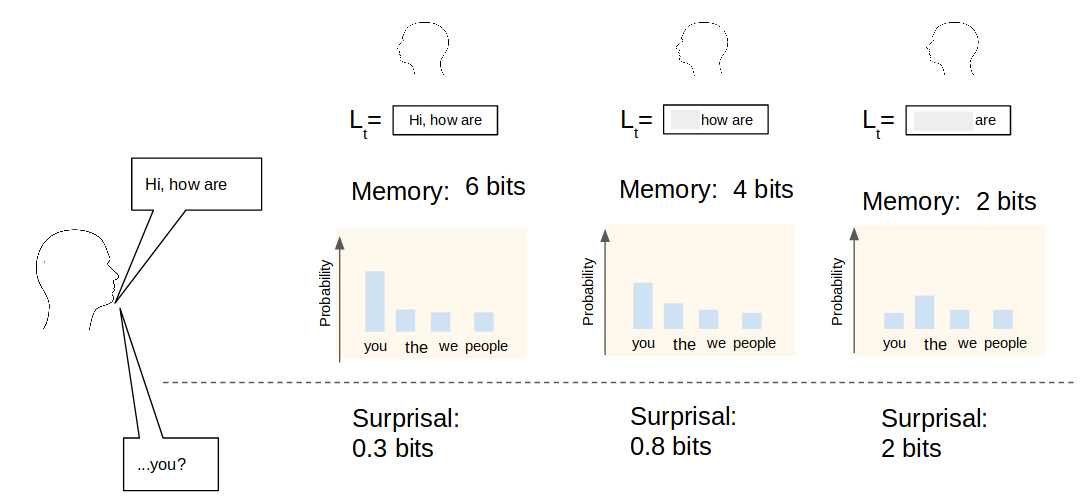
\includegraphics[width=0.9\textwidth]{figures-gdrive/communication.png}
%	\caption{Memory and language comprehension. (1) A speaker produces a sequence of words. (2) A listener maintains a representation of the words received so far. The listener can represent these at higher (left) or lower (right) levels of precision. (3) Throughout communication, the listener generates probabilistic expectations about the next word. Higher precision of memory representations leads to more precise predictions. (4) When receiving the next word, the listener incurs surprisal depending on the predictions. Higher levels of fidelity in memory lead to lower surprisal on average. \jd{what do the numbers (1) (2) etc refer to? also: image is blurry, at least on my screen}\note{make reference to $L_t$ inside the caption. you and the surprisals visually better aligned. maybe can color-code? } \mhahn{problem suggests that memory has to be contiguous substrings}}
%	\label{fig:communication}
%\end{figure}

We begin developing our model by considering the process of language comprehension illustrated in Figure~\ref{fig:communication}, where the listener Alice is processing a stream of words uttered by an interlocutor Bob (Figure~\ref{fig:communication}). 

Experimental research has established three properties of online language comprehension: (1) listeners maintain some information about the words received so far in incremental memory, (2) listeners form probabilistic expectations about the upcoming words, and (3) words are easy to process to the extent that they are predictable based on a listener's memory of words received so far. (TODO REFS)\jdegen{this invites the question of whether anything you're about to show us holds if these assumptions aren't in fact warranted. eg, people love to argue about whether listeners *really* predict}

We formalize these three observations into postulates intended to provide a simplified picture of what is known about online language comprehension. Consider a listener comprehending a sequence of words $w_1, \dots, w_t, \dots, w_n$, at an arbitrary time $t$.
\begin{enumerate}
    \item Comprehension Postulate 1 (Incremental memory). At time $t$, the listener has an incremental \key{memory state} $m_t$ that contains her stored information about previous words. The memory state is given by a \key{memory encoding function} $M$ such that $m_t = M(w_{t-1}, m_{t-1})$.
    \item Comprehension Postulate 2 (Incremental prediction). The listener has a subjective probability distribution at time $t$ over the next word $w_t$ as a function of the memory state $m_t$. This probability distribution is denoted $P(w_t|m_t)$.
    \item Comprehension Postulate 3 (Linking hypothesis). Processing a word $w_t$ incurs difficulty proportional to the \key{surprisal} of $w_t$ given the memory state $m_t$:
    \begin{equation}
    \label{eq:lossy-surp}
    \text{Difficulty} \propto -\log P(w_t | m_t).
\end{equation}
\end{enumerate}
The claim that processing difficulty should be directly proportional to surprisal comes from \key{surprisal theory} \citep{hale2001probabilistic,levy2008expectation}, an established psycholinguistic theory that can capture reading time effects related to garden-path disambiguation, antilocality effects, and effects of syntactic construction frequency. Surprisal is a robust linear predictor of reading times in large-scale eye-tracking studies based on naturalistic text \citep{smith-effect-2013,goodkind-predictive-2018}, and effects of surprisal have been observed for units as small as phonemes \citep{}.

Our expression~(\ref{eq:lossy-surp}) differs from the usual formulation of surprisal theory in that we consider predictability based on a (potentially lossy or noisy) memory representation $m_t$, rather than predictability based on the true complete context $w_1, \dots, w_{t-1}$. The generalization to lossy memory representations is necessary to capture empirically observed effects of memory limitations on language processing, such as dependency locality and structural forgetting \citep{futrell2020lossy}. For other ways of capturing effects of both memory limitations and probabilistic expectations, see \citet{demberg-incremental-2013} and \citet{rasmussen-2017-left}.


In this work, we are interested in using theories of processing difficulty to derive predictions about languages as a whole, not about individual words or sentences. Therefore, we need a measure of the processing difficulty associated with a language as a whole. For this, we consider the \emph{average} surprisal per word in the language. We call this quantity the \key{average surprisal} of a language given a memory encoding function $M$, denoted $S_M$.

Crucially, the listener's ability to predict upcoming words accurately depends on how much she remembers about previous words. As the precision of her memory increases, the accuracy of her predictions also increases, and the average surprisal $S_M$ for each incoming word decreases. Taking an information-theoretic perspective, we can think about the amount of information (measured in bits) about previous words stored in the listener's memory state. This quantity of information is given by the \key{entropy} of the memory state, which we denote $H_M$. As the listener stores more and more bits of information about the previous words her memory state, she can achieve lower and lower surprisal values for the upcoming words. This trade-off between memory and surprisal is the main object of study in this paper.

The \key{memory--surprisal trade-off curve} answers the question: 
for a given amount of information about previous words $H_M$ stored in the listener's memory state, what is the lowest achievable average surprisal $S_M$? Two example trade-off curves are shown in Figure~\ref{fig:examples}. In general, as the listener stores more information about previous words in her memory state, her lowest achievable average surprisal must go down. So the curve is always monotonically decreasing. However, the precise shape of the trade-off curve depends on the structure of the language being predicted. For example, Figure~\ref{fig:examples} shows how two processes might engender different trade-off curves, with Language $A$ allowing more favorable trade-offs than Language $B$. That is, for Language $A$, it is possible to achieve lower processing difficulty while investing less memory resources than in Language $B$.

\begin{figure}
\centering
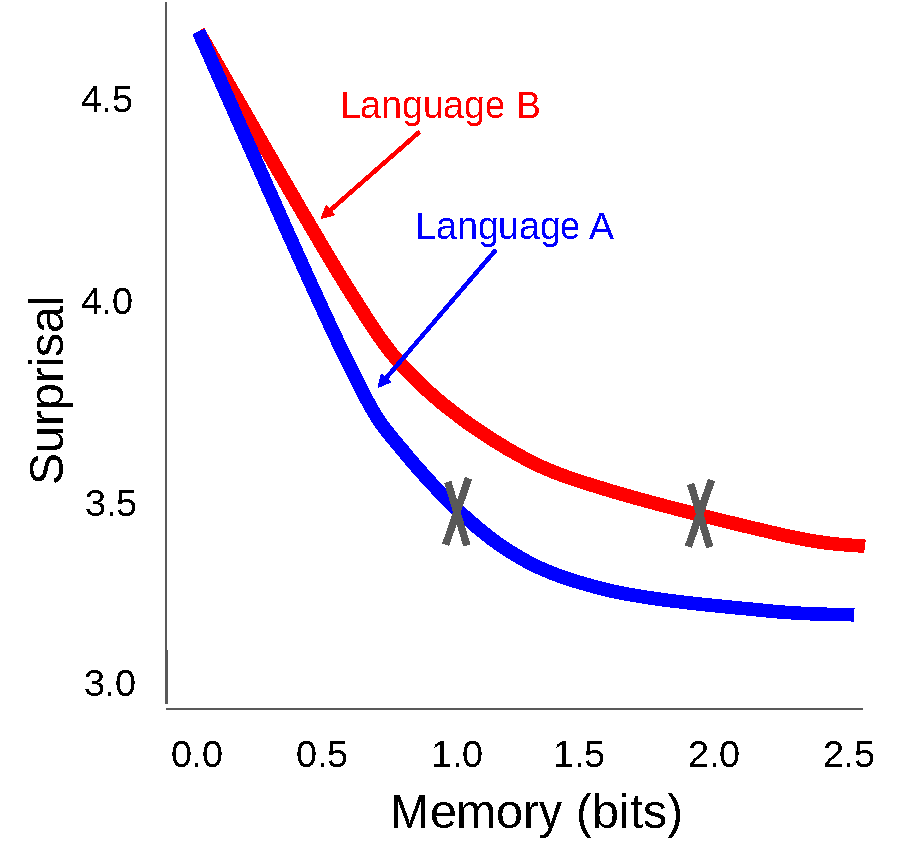
\includegraphics[width=0.5\textwidth]{figures-gdrive/tradeoff-schematic.pdf}
\caption{Example memory--surprisal trade-off curves for two languages, $A$ and $B$. Achieving an average surprisal of 3.5 bits requires storing at least 1.0 bits in language $A$, while it requires storing 2.0 bits in language $B$. Language $B$ has a steeper memory--surprisal trade-off than Language $A$, and requires less memory resources to achieve the same level of processing difficulty.}
\label{fig:examples}
\end{figure}

\subsection{Main hypothesis}

Now that we have conceptually introduced the memory--surprisal trade-off, we can state the main hypothesis of this work:

\paragraph{Main hypothesis.}  Natural language is characterized by a distinctively steep memory--surprisal trade-off curve.\jdegen{why?}

A steep trade-off curve corresponds to memory-efficiency, in the sense that it is possible to achieve a low level of processing difficulty (average surprisal $S_M$) while storing a relatively small amount of information about previous words (entropy of memory $H_M$).
We hypothesize that this property is reflected both in the grammatical structure of languages and in usage preferences.


\subsection{Formal definition of the memory--surprisal trade-off}
\label{sec:formal-tradeoff}

Here we provide the technical definition of the memory--surprisal trade-off curve and relate it to concepts from information theory, rate--distortion theory, and statistical complexity theory.

Let $W$ be a stochastic process\footnote{We will use $W$ to represent languages, and we will construct $W$ to be stationary. Large natural language texts are known to be neither stationary nor ergodic \citep{debowski}. However, we are interested in explaining grammatical properties of languages, which mostly involve constraints among words within sentences, not within large texts as a whole. Therefore, we will represent a language using a stochastic process consisting of repeated independent samples from a distribution over sentences. This stochastic process is both stationary and ergodic.} generating a stream of symbols called words, indexed as $w_1, \dots, w_t$.\footnote{We call these symbols words, but note that our mathematical treatment applies for \emph{any} decomposition of a sentence into a sequence of symbols---the symbols could represent phonemes, syllables, morphemes, words, phrases, etc.} Let $M$ be a memory encoding function. The \key{average surprisal} of the process $W$ under the memory encoding function $M$ is
%\mhahn{We have to decide whether we want the process to be stationary and infinite, or instead semi-infinite. The formalization of the locality theorem assumes it is stationary and infinite in both directions.}
\begin{equation}
%    S_M \equiv \lim_{t \rightarrow \infty} H[w_t | m_t],
    S_M \equiv H[w_t | m_t],
\end{equation}
where the notation $H[\cdot | \cdot]$ indicates conditional entropy \citep[][p. 17]{cover2006elements}:
\begin{equation}
    H[w_t|m_t] \equiv -\sum_{w_t,m_t} P(m_t) P(w_t|m_t) \log P(w_t|m_t).
\end{equation}
%\jdegen{maybe it's worth providing the definition first but to tell readers to skip this subsection and go to the informal/intuitive explanation that currently comes before this?}
The lowest possible average surprisal for $W$ that can be attained by any memory encoding function is called the \key{entropy rate} of $W$ \citep[][pp. 74--75]{cover2006elements}:
\begin{equation}
    \label{eq:entropy-rate}
    S_\infty \equiv \lim_{t \rightarrow \infty} H[w_t | w_1, \dots, w_{t-1}].
\end{equation}
 The entropy rate of a stochastic process is the irreducible unpredictability of the process: the extent to which a stream of symbols remains unpredictable even for a predictor with unlimited resources. 
 We use the notation $S_\infty$ to suggest this idea of unlimited resources.
 The entropy rate of natural language text has been studied by \citet{shannon1951entropy}, \citet{takahira}, and \citet{bentz}. 
 The average surprisal $S_M$ can also be called a \key{cross entropy rate}.  Because the memory state $m_t$ is a function of the previous words $w_1, \dots, w_{t-1}$, we can prove by the Data Processing Inequality \citep[][pp. 34--35]{cover2006elements} that the entropy rate must be less than or equal to the average surprisal for any memory encoding function $M$:
\begin{equation}
    \label{eq:entropy-rate-dpi}
    S_\infty \le S_M.
\end{equation}
If the memory state $m_t$ stores all information about the previous words $w_1, \dots, w_{t-1}$, then we have $S_M = S_\infty$.
Based on Eq.~\ref{eq:entropy-rate-dpi}, we can write the average surprisal $S_M$ as a sum of two non-negative terms,
\begin{equation}
    S_M = S_\infty + d_M,
\end{equation}
where $d_M$ is \key{memory distortion}: the extra surprisal incurred in addition to the unavoidable surprisal $S_\infty$, owing to the lossiness of the memory encoding function $M$. 
The memory distortion $d_M$ is formally a Kullback-Leibler (KL) divergence:
\begin{equation}
    \label{eq:memory-distortion}
    d_M = \lim_{t \rightarrow \infty} D_{\text{KL}} [ p(w_t | w_1, \dots, w_{t-1}) || p(w_t | m_t)].
\end{equation}
Finding a memory encoding function $M$ to minimize $S_M$ is equivalent to minimizing the memory distortion $d_M$.

Having defined average surprisal and related concepts, we now turn to the question of how to define memory capacity. The average amount of information stored in the memory states $m_t$ is the entropy of the stationary distribution over memory states, $H_M$:
\begin{align}
    \label{eq:memory-entropy}
    H_M &\equiv H[m] \\
    &= - \sum_m p(m) \log p(m).
\end{align}
The minimum value of $H_M$ that achieves $S_M = S_\infty$ is called the \key{statistical complexity} of the process $W$ \citep{shalizi2001computational}. The statistical complexity of natural language has been studied by \citet{hahn2019neural}. We will be imposing bounds on $H_M$ and studying the resulting values of $S_M$. 

\begin{definition}
The \key{memory--surprisal trade-off curve} for a process $W$ is the lowest achievable average surprisal $S_M$ for each value of $H_M$. Let $R$ denote an upper bound on the memory entropy $H_M$; then the memory--surprisal trade-off curve as a function of $R$ is given by
\begin{equation}
    \label{eq:ms-formal}
    D(R) \equiv \min_{M : H_M \le R} S_M,
\end{equation}
where the minimization is over all memory encoding functions $M$ whose entropy $H_M$ is less than or equal to $R$.
\end{definition}

The memory state $m_t$ is generally a lossy representation of the true context of words $w_1, \dots, w_{t-1}$, meaning that $m_t$ does not contain all the possible information about $w_1, \dots, w_{t-1}$. The mathematical theory of lossy representations is \key{rate--distortion theory} \citep[for an overview and key results, see][pp. 301--347]{cover2006elements}; this theory has seen recent successful application in cognitive science and linguistics as a model of rational action under resource constraints \citep{sims,gershman,zaslavsky2018efficient}. Rate--distortion theory studies curves of the form of Eq.~\ref{eq:ms-formal}, which quantify trade-offs between utility (`distortion') and information (`rate'). Our memory--surprisal trade-off curve is a distortion--rate curve, with $H_M$ as the rate and $S_M$ as the distortion. It differs from the typical curve studied in rate--distortion theory in that we define rate using entropy, rather than mutual information \citep[see][for a discussion of some of the consequences of this formulation]{strouse-deterministic-2017}. 
Our theoretical results still hold if we were to define rate using mutual information (see SI Section REF).


\subsection{Information locality}
\label{sec:infoloc}

The shape of the memory--surprisal trade-off is determined in part by the grammatical structure of a language.
Some languages enable more efficient trade-offs than others by forcing a listener to store more bits in memory to achieve the same level of average surprisal.

Here, we will demonstrate that the memory--surprisal trade-off is optimized by languages with word orders exhibiting a property called \key{information locality}. Information locality means that words that depend on each other statistically are located close to each other in time. We will argue that information locality generalizes the well-known word order principle of dependency locality.

We will make our argument by defining a lower bound on the memory--surprisal trade-off curve (Eq.~\ref{eq:ms-formal}). This lower bound represents an unavoidable cost associated with a certain level of memory usage $H_M$; the true average surprisal $S_M$ might be higher than this bound. 

Our argument will make use of a quantity called \key{mutual information}. Mutual information is the most general measure of statistical association between two random variables. The mutual information between two random variables $X$ and $Y$, conditional on a third random variable $Z$, is defined as:
\begin{align}
\label{eq:mi}
    I[X:Y|Z] &\equiv \sum_{x,y,z} P(x,y,z) \log \frac{P(x,y|z)}{P(x|z)P(y|z)} \text{ bits} \\
    \nonumber
    &= H[X|Z] - H[X|Y,Z] \\
    \nonumber
    &= H[Y|Z] - H[Y|X,Z].
\end{align}
Mutual information is always non-negative. It is zero when $X$ and $Y$ are conditionally independent given $Z$, and positive whenever $X$ gives any information that makes the value of $Y$ more predictable, or vice versa. 


\begin{figure}
	(a)
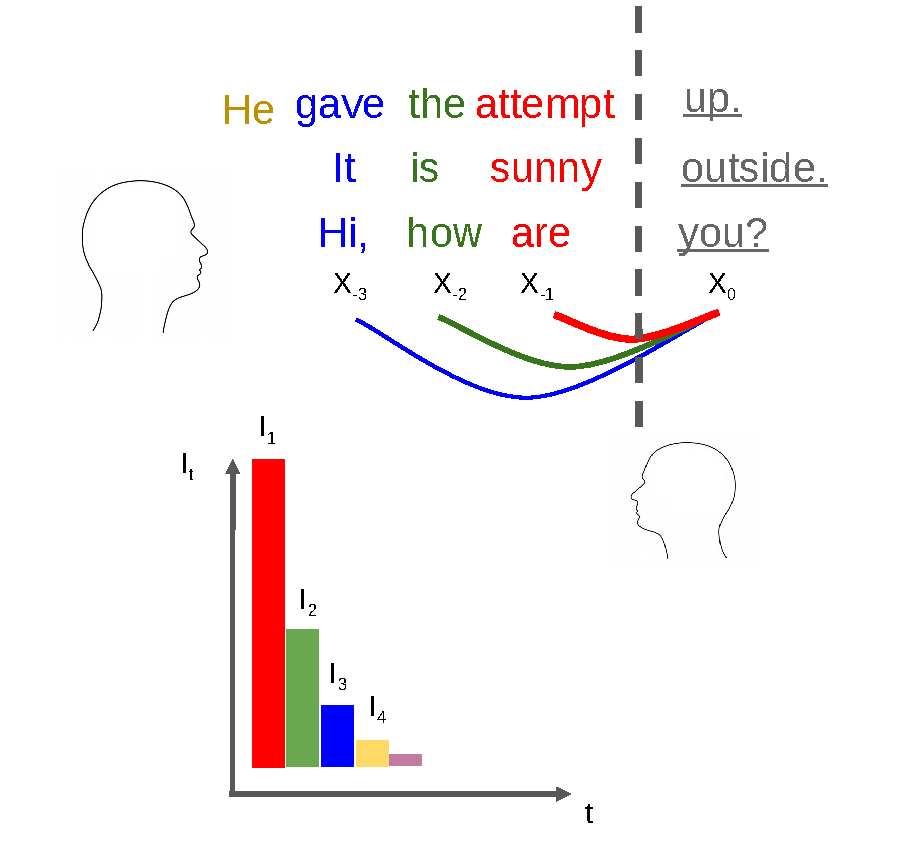
\includegraphics[width=0.4\textwidth]{figures-gdrive/mi-distance.pdf}
	(b)
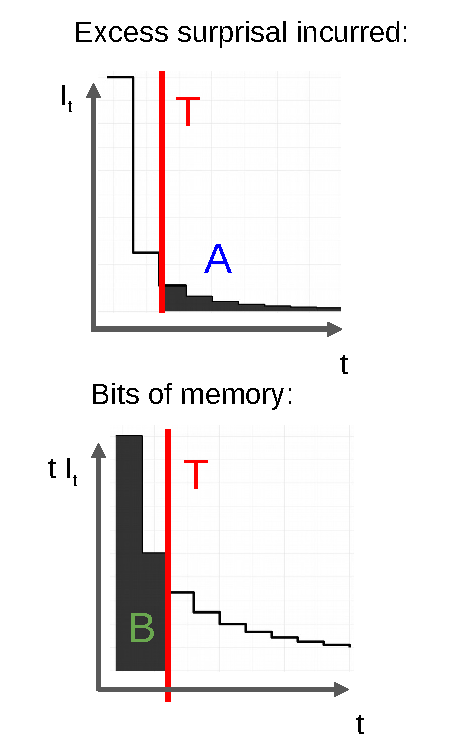
\includegraphics[width=0.25\textwidth]{figures-gdrive/theorem.pdf}
	\caption{
		(a) Conditional mutual information $I_t$ captures how much predictive information about the next word is provided, on average, by the word $t$ steps in the past.
		(b) Here we illustrate our theoretical result. We plot $I_t$ (top) and $tI_t$ (bottom) as functions of $t$. For any choice of $T$, a listener using $B$ bits memory (bottom) to represent prior observations will incur at least $A$ bits of extra surprisal beyond the entropy rate (top). 
}\label{fig:theorem}
\end{figure}





We will study the mutual information structure of natural language sentences, and in particular the mutual information between words at certain distances in linear order. We define the notation $I_t$ to mean the mutual information between words at distance $t$ from each other, conditional on the intervening words:
\begin{align}
    \nonumber
    I_t &\equiv I[w_t : w_0 | w_1, \dots, w_{t-1}] \\
    \nonumber
    &= H[w_t | w_1, \dots, w_{t-1}] - H[w_t | w_0, \dots, w_{t-1}].
\end{align}
This quantity, visualized in Figure~\ref{fig:theorem}(a), measures how much predictive information is provided about the current word by the word $t$ steps in the past.
It is a statistical property of the language, and can be estimated from large-scale text data.

Equipped with this notion of mutual information at a distance, we can now state our theorem:
\begin{thm}\label{prop:suboptimal}(Information locality bound) For any positive integer $T$, let $M$ be a memory encoding function such that
\begin{equation}
\label{eq:memory-bound}
H_M \le \sum_{t=1}^T t I_t.    
\end{equation}
Then we have a lower bound on the average surprisal under the memory encoding function $M$:
\begin{equation}
\label{eq:surprisal-bound}
S_M \ge S_\infty + \sum_{t=T+1}^\infty I_t.
\end{equation}
\end{thm}
A formal proof, relying only on the stationarity of the stochastic process, is given in Appendix Section X. 

\paragraph{Interpretation} The theorem means that a predictor with limited memory capacity will always be affected by surprisal cost arising from long-term statistical dependencies of length greater than $T$, for some finite $T$. This is why we call the result `information locality': processes are easier to predict when most statistical dependencies are short-term (shorter than $T$). Below we explain in more detail how this interpretation matches the mathematics of the theorem.

The quantities in the theorem are illustrated visually in Figure~\ref{fig:theorem}. Eq.~\ref{eq:memory-bound} describes a memory encoding function which has enough capacity to remember the relevant information from at most $T$ words in the immediate past. The minimal amount of memory capacity which would be required to retain this information is the sum $\sum_{t=1}^T t I_t$, reflecting the cost of holding $I_t$ bits in memory for $t$ timesteps up to $t=T$. 

The information locality bound theorem says that the surprisal cost for this memory encoding function is at least $S_\infty + \sum_{t=T+1}^\infty I_t$ (Eq.~\ref{eq:surprisal-bound}). The first term $S_\infty$ is the entropy rate of the process, representing the bits of information in the process which could not have been predicted given any amount of memory. The second term $\sum_{t=T+1}^\infty I_t$ is the sum of all the relevant information contained in words \emph{more} than $T$ timesteps in the past (see Figure~\ref{fig:theorem}(b)). These correspond to bits of information in the process which \emph{could have} been predicted given infinite memory resources, but which were not, due to the limit on memory usage.

The theorem gives a lower bound on the memory--surprisal trade-off curve, meaning that there is no memory encoding function with capacity $H_M$ which achieves lower average surprisal than Eq.~\ref{eq:surprisal-bound}. In terms of psycholinguistics, if memory usage is bounded by Eq.~\ref{eq:memory-bound}, then processing cost of at least Eq.~\ref{eq:surprisal-bound} is inevitable.

\begin{figure*}
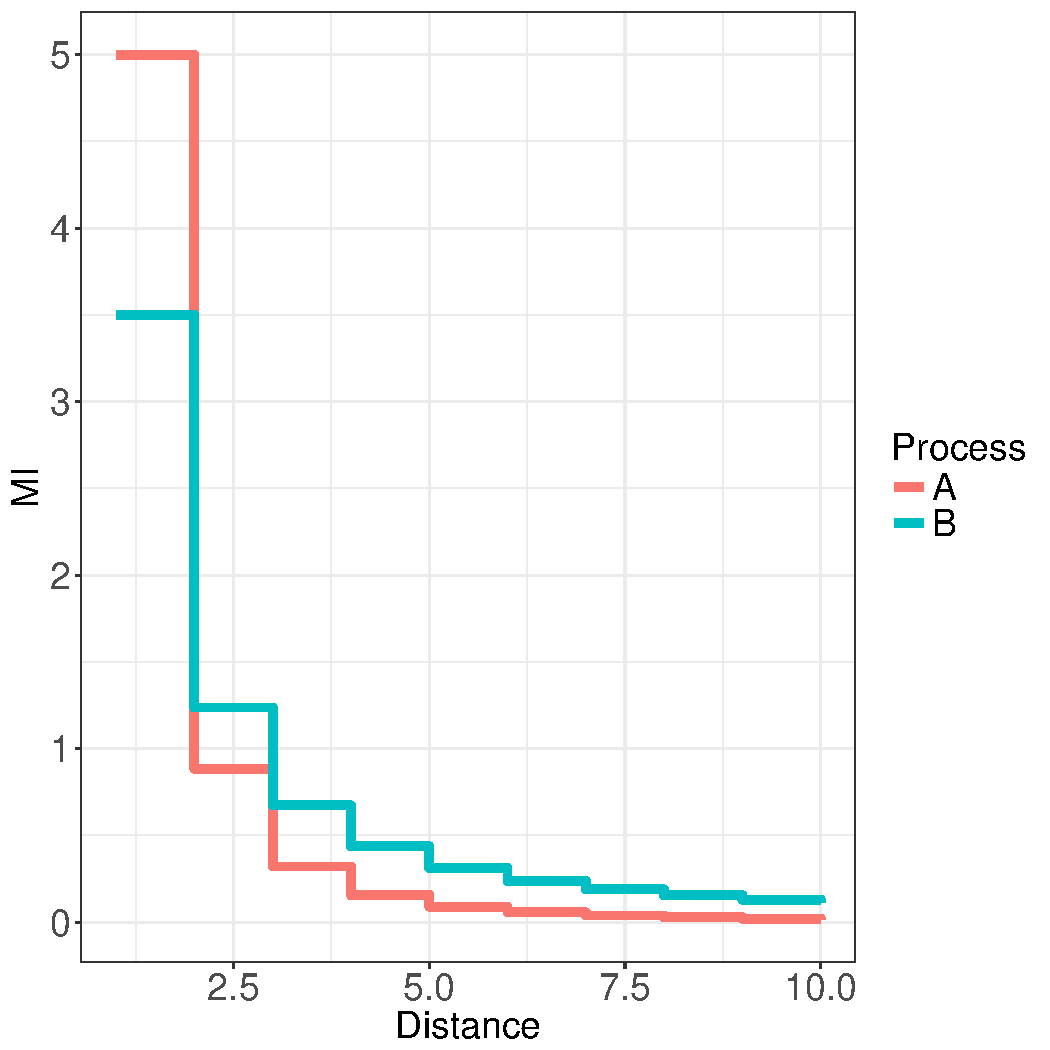
\includegraphics[width=0.45\textwidth]{figures/decay.pdf}
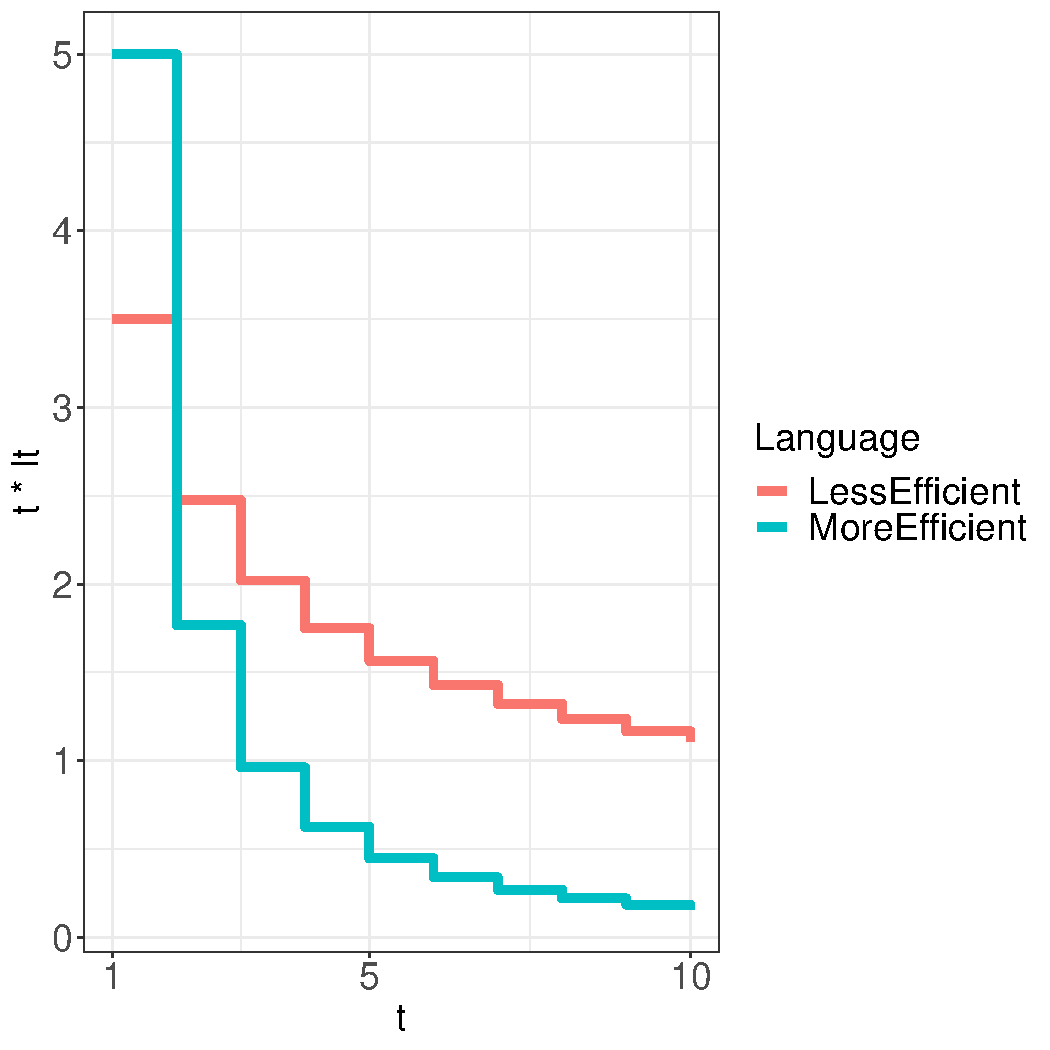
\includegraphics[width=0.45\textwidth]{figures/memory.pdf}
%
	\caption{Left: $I_t$ as a function of $t$, for two different processes. $I_t$ decays faster for the red process: Predictive information about the present observation is concentrated more strongly in the recent past. Left: $t \cdot I_t$ as a function of $t$ for the same processes. \mhahn{x-axis should be integers. axis labels match captions.} }\label{fig:basic}
\end{figure*}

\begin{figure}
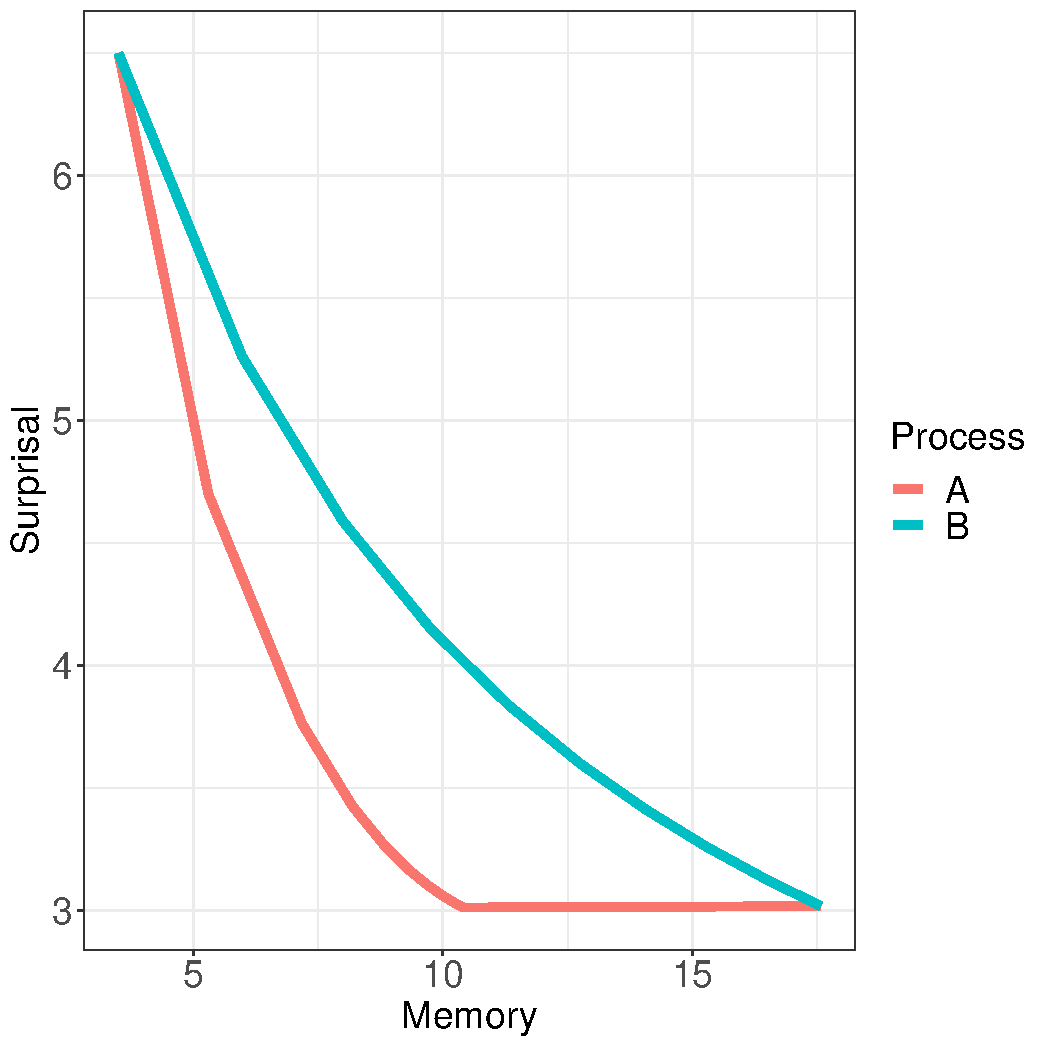
\includegraphics[width=0.45\textwidth]{figures/listener-tradeoff.pdf}
	\caption{Listener's memory-surprisal tradeoff for the two processes in Figure~\ref{fig:basic}. Recall that the red process had a faster decay of conditional mutual information. Correspondingly, this figure shows that a listener can achieve lower surprisal at the same level of memory load. \mhahn{add missing line at bottom}}\label{fig:listener-tradeoff}
\end{figure}

Eq.~\ref{eq:memory-bound} means that maintaining long-term dependencies requires higher memory usage. Carrying the same amount of information over longer distances requires more memory; this fact is reflected in the factor $t$ inside each term of the sum. 
The result is that modeling long-term statistical dependencies is more costly in terms of memory usage than modeling shorter ones.
The information locality bound theorem demonstrates in a highly general way that language comprehension requires less memory resources when statistical dependencies are mostly short-term. 

Because processing long-term dependencies requires higher memory usage, the theorem also implies that a language will be easier to process when most of the predictive information about a word is concentrated close to that word in time---that is, when $I_t$ falls off rapidly as $t \rightarrow \infty$. When memory capacity is limited, then there must be some timescale $T$ such that a listener appears to be affected by excess surprisal arising from statistical dependencies of length greater than $T$. A language avoids such cost to the extent that it avoids dependencies with a time-span larger than $T$.

We illustrate the theorem in Figure~\ref{fig:basic}.
We consider two processes $A$ and $B$, where $I_t := 5t^{-1.5}$ for $A$ and $I_t := 3.5 t^{-2.5}$ for $B$.
The curves of $I_t$, as a function of the distance $t$, are shown in Figure~\ref{fig:basic} (left).
In both cases, $I_t$ converges to zero as $t$ grows to infinity. 
However, $I_t$ decays more quickly for Process A (red).
This means that predictive information about an observation is concentrated more strongly in the recent past.
In Figure~\ref{fig:basic} (right), we show $t\cdot I_t$ as a function of $t$.
Note that the area under the curve is equal to (\ref{eq:memory-bound}).
This area is smaller for the red process, as $I_t$ decays more quickly there.  




